\chapter{Implementation \label{cha:chapter5}}

This chapter describes the implementation details, including the structural decisions and  encountered development challenges, of the Rollup System based on the system described at \ref{sec:2_adspProject}. Figure \ref{fig:fig:5_drawings-final_rollup_archotecture.png} shows the system's final architecture, clearly distinguishing Layer 1 and Layer 1 components and showing the interactions between them.

\begin{figure}[ht]
	\centering
	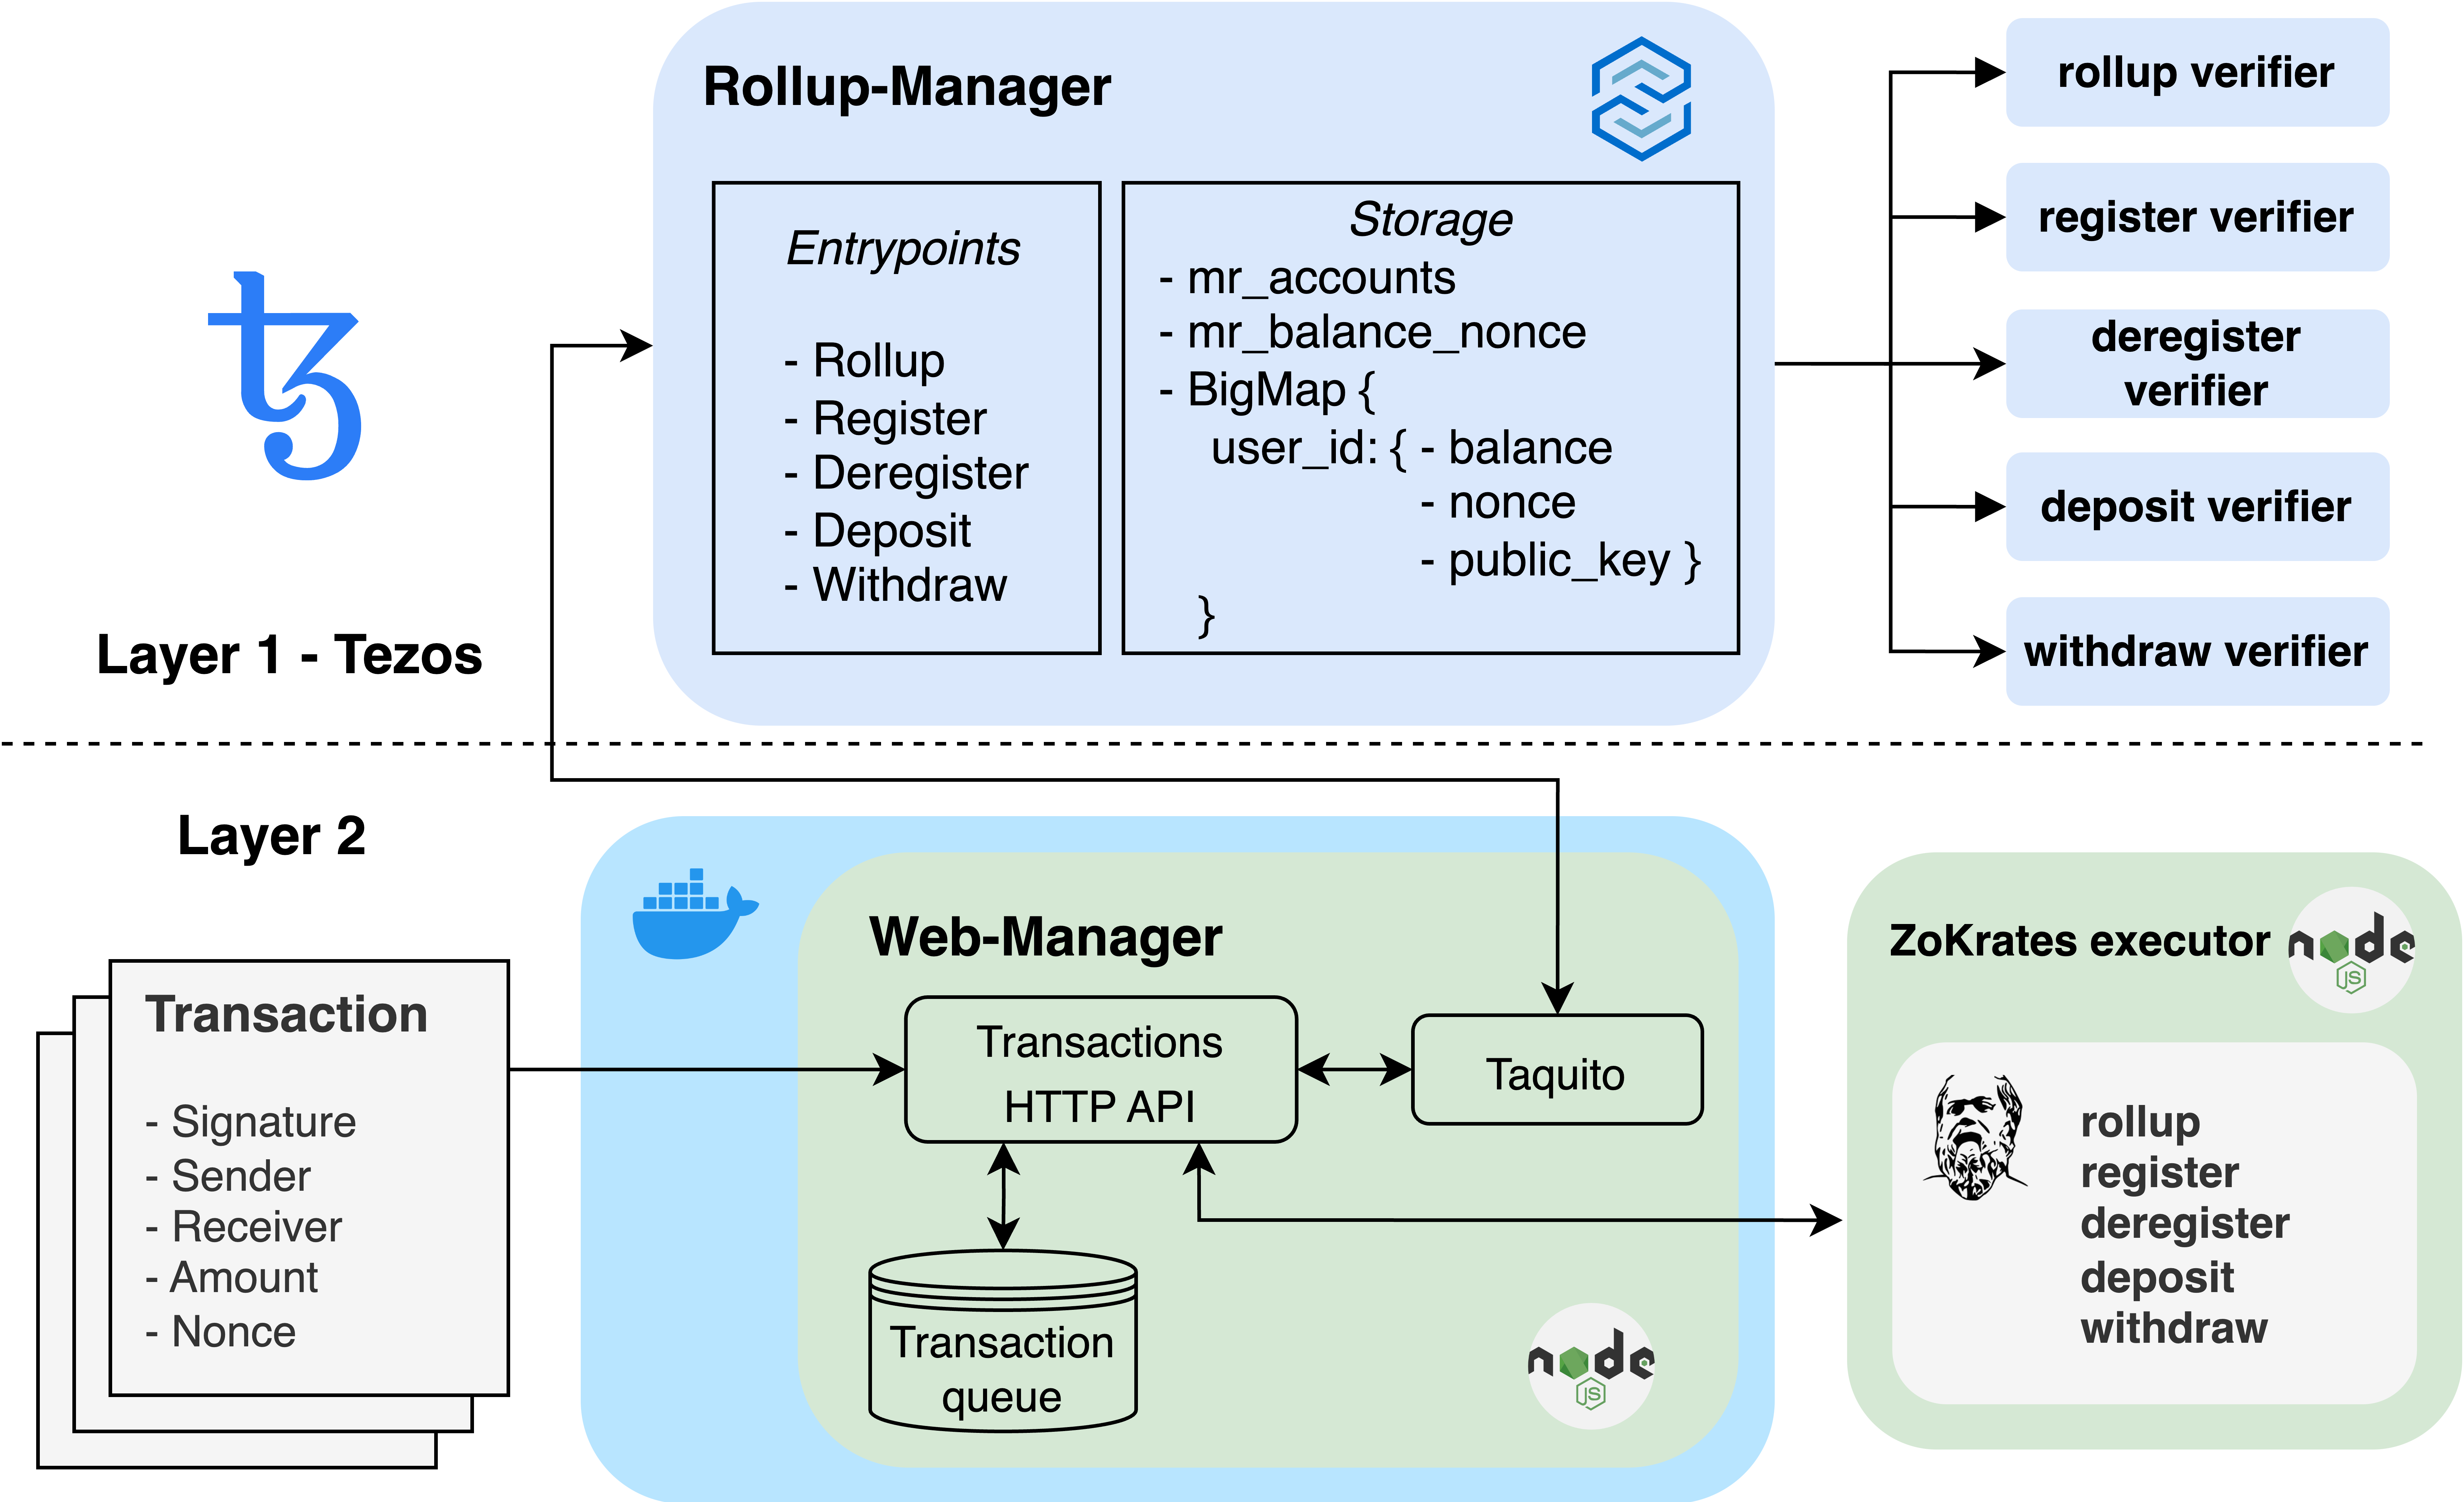
\includegraphics[width=0.9\columnwidth]{5_drawings-final_rollup_architecture.png}
	\caption[Rollup Architecture]{Architecture of the Rollup System.}
	\label{fig:fig:5_drawings-final_rollup_archotecture.png}
\end{figure}

\section{Technologies\label{sec:technologies}}

The blockchain components are constructed utilizing the Tezos blockchain\footnote{\url{https://tezos.com/}} and the SmartPy\footnote{\url{https://smartpy.io/}} smart contract language. The Rollup System is deployed on the Tezos Ghostnet test network.

To design and build the Layer 2 components, web servers are developed using nodejs and Typescript running in Docker containers. The implementation of Rollup programs is achieved through the utilization of the ZoKrates toolbox\footnote{\url{https://github.com/ZoKrates/ZoKrates}}, a comprehensive zk-SNARKs toolkit designed to facilitate the creation of verifiable computation programs.

The interaction between the Layer 2 and Layer 1 is made possible through the utilization of the Taquito\footnote{\url{https://tezostaquito.io/}} library, a TypeScript library that provides a simple interface for interacting with the Tezos blockchain.

Those technologies were already decided at the time of the project's inception, as they were the most suitable for the project's objectives. The Tezos blockchain was chosen due to its easy development and deployment, as well as the missing Layer 2 solutions.

\section{Repeated Transactions Attack}
\label{sec:repeatedtransactionsattack}

To mitigate the risk of an attacker initiating repeated transactions, the nonce mechanism has been introduced: each account holds a nonce, stored on Layer 1. When a transaction is submitted, it must include a nonce incremented by one, thereby facilitating the validation of transaction execution history.

Within the ZoKrates environment, proving the usage of updated balances and nonces necessitates computation of a merkle tree for the provided balance and nonce lists. This implies calculating two full binary trees, thereby increasing complexity. A workaround involves concatenating and hashing balances and nonces for individual users, forming a single merkle tree of these concatenated values. This approach incurs only the complexity of the concatenation function, involving a number of hashes equivalent to the number of accounts, but still allowing to proof that the balances and nonces are updated.

Changes were introduced to the rollup execution to incorporate the computation of new nonces alongside new balances. It's essential that ZoKrates receives transactions ordered by nonce for each user. While transactions from diverse users can be received, those from a single user must be ordered by nonce. The algorithm for verifying transaction nonces and calculating new nonces is as follows:
\begin{itemize}
	\item Initialize \textit{nonce\_array} and \textit{balance\_array}, with the current nonces and balances of all users;
	\item Iterate through the transactions:
	      \begin{itemize}
		      \item Check in \textit{nonce\_array} if the transaction nonce equals the sender's nonce plus one;
		      \item If true:
		            \begin{itemize}
			            \item Increment senders's nonce in array \textit{nonce\_array};
			            \item Decrement sender's balance in array \textit{balance\_array};
			            \item Increment receiver's balance in array \textit{balance\_array};
			            \item Proceed to next transaction;
		            \end{itemize}
		      \item If false:
		            \begin{itemize}
			            \item Fail program execution.
		            \end{itemize}
	      \end{itemize}
\end{itemize}

This approach accommodates multiple transactions from the same user, preventing duplicate transaction execution.

The rollup execution complexity experiences minimal rise, as the nonce check coincides with balance calculation in the same loop, facilitating direct array access and preserving an O(n) complexity.

\section{Hash Function}

Hash functions play a crucial role in the Rollup execution process. They are extensively used for various tasks such as creating Merkle Trees, concatenating balances and nonces, and verifying signatures. One widely supported hashing function in this context is SHA-256. The initial implementation of the Rollup system employed the SHA-256 function provided by the ZoKrates toolbox. However, as demonstrated in Section \ref{subsec:6_hashfunc}, the use of this function introduces a significant number of constraints to the compiled Zokrates program, resulting in exponential complexity during execution. This inefficiency arises from the fact that classical cryptographic schemes predominantly consist of boolean operations, which become inefficient within a ZK-SNARK circuit \cite{belles-munoz_twisted_2021}.

A more recent hash function, known as Poseidon \cite{grassi_poseidon_nodate}, has been developed with a specific focus on efficiency within zk-SNARK circuits. By transitioning the Rollup system's hash function from SHA-256 to Poseidon, the number of constraints added to the program has been reduced by a factor of 100.

Notably, the adoption of the Poseidon hash function necessitates a revision of the system storage. While SHA-256 operates on 256-bit blocks, Poseidon operates on field sizes defined by the underlying elliptic curve. Additionally, considering the process of signature verification, the payload of a signed message must be hashed to fit a predetermined size prior to verification. In the case of Zokrates signature verification, which expects 512 bits of data, padding must be added after hashing the payload with Poseidon. This is due to the fact that the bls12\_381 curve on ZoKrates operates on a 254-bit field size. To meet the expected size, a padding of 258 bits, filled with zeros, is appended to the right of the payload's hash.

The signature verification, done for each transaction, still uses sha2 hashes, as enforced by Ed25519 standard. This means that the signature verification may be considered a bottleneck for the system, as better shown in Section \ref{subsec:6_zokratesperf}. A future and possible s

\section{Proof Reduction and Compression \label{sec:5_redandcompr}}

When setting up ZoKrates' private and verification keys, it's important to remember that the key sizes depend on the number of outputs in the ZoKrates program. When you run a Rollup, these outputs represent the updated Merkle Tree that combines balances and nonces, along with the list of balances and nonces. These values are crucial for updating the inner storage of the Manager Smart Contract on Layer 1. As explained in Section \ref{sec:3_smartContractsRequirements}, everything sent to the blockchain must be no more than 32768 bytes in total.

As more users and transactions come into play, proof size grows, causing the keys to also become larger. Unfortunately, this situation makes it impossible to send the proof to the Rollup Smart Contract, which essentially breaks the system. To address this, a potential solution is to find a way to shrink and compress the outputs produced by the zokrates program.

Implementing this solution would allow the system to handle a higher number of users and transactions since the proof size would be smaller. Table \ref{tab:5_keyandproofsize} shows an example of what the algorithm could achieve in a system with 1024 users and 3 transactions

\begin{table}
	\centering
	\begin{tabular}{|l|c|c|}
		\hline
		                 & Without algorithm & With algorithm \\
		\hline
		Verification key & 462KB             & 5,5KB          \\
		\hline
		Proof            & 151KB             & 2,1KB          \\
		\hline
	\end{tabular}
	\caption[Key and Proof size]{Key and Proof size comparison using 1024 users and 3 transactions}
	\label{tab:5_keyandproofsize}
\end{table}

\subsection{Proof Reduction}

To achieve a reduction in the number of outputs from the ZoKrates program, a change is made in the program's logic. Instead of returning the entire list of balances and nonces, the program only returns the altered balances and nonces. This adjustment introduces the requirement for an index that can be used to identify users in the list.

For every transaction, certain information needs to be returned: the sender's index, balance, and nonce, as well as the receiver's index and balance. In a hypothetical rollup system with 4096 users and 128 transactions per rollup, the outputs of the ZoKrates program shrink from 8193 to 641 (inclusive of the Merkle Root). This reduction significantly cuts down the proof size. Notably, in a Rollup system, many users remain inactive, participating infrequently in the rollup. This dynamic creates a considerable gap between the registered user count and the number of transactions, which enables this mechanism.

Furthermore, this approach proves more advantageous when a single user initiates multiple transactions to the same recipient, as the sender's index and balance are only returned once.

\subsection{Proof Compression \label{subsec:5_compression}}

ZoKrates allows operating on fields of size 254 bits. The proof itself is made up of entries in these fields, no matter the original type of value. Even a simple boolean or a 254-bit value gets represented using just one field entry. This applies to lists of changed indexes, balances, and nonces too. When returning the list of modified indexes, balances and nonces each of them will occupy a single field value for just 32 bits of information.

By combining indexes, balances, and nonces into one field value, we can fit more info in a single entry. This merging cuts down the number of field entries returned from the ZoKrates program, which in turn shrinks the proof size. Here's a snippet of how this compression works within the ZoKrates program:

\begin{lstlisting}[language=C++]
field[NUM_TRANSACTIONS] mut result = [0; NUM_TRANSACTIONS];
for u32 i in 0..NUM_TRANSACTIONS {
  // Calculate new balances and nonce
  ......
  // Compress indexes, balances, and nonces
  bool[32] index_send_bits = u32_to_bits(index_sender);
  bool[32] balance_send_bits = u32_to_bits(balance_sender);
  bool[32] nonce_send_bits = u32_to_bits(nonce_sender);
  bool[32] index_rec_bits = u32_to_bits(index_receiver);
  bool[32] balance_rec_bits = u32_to_bits(balance_receiver);
  bool[254] joined = [
    ...index_send_bits, ...balance_send_bits,
    ...nonce_send_bits, ...[false; 94],
    ...index_rec_bits, ...balance_rec_bits
  ];
  result[i] = pack(joined);
}
\end{lstlisting}

This process returns one field value for each transaction. The first 96 bits hold sender-related data, followed by a 94-bit padding, and then 64 bits for receiver-related data.

Another possible way to improve this mechanism is by concatenating all the data into one bit array, and then taking 254-bit chunks from it to create field values, saving up in the padding bits.

To get back the original values, the Smart Contract needs to decompress the field data applying the reverse algorithm. At the moment, the ability to retrieve the 32 bit chunks from the field values is there, but the current SmartPy version lacks converting from Bytes to Nat. When that feature comes in, it will be possible to restore original values from field values. The upcoming benchmarks will also account for an estimated gas cost of this value conversion by adding an useless conversion.

\section{Storage\label{sec:5_storage}}

Initially, the storage was designed with the intention of accommodating a limited number of users, employing a standard Map. Standard maps in Tezos are always deserialized at every contract execution, even if the elements of the map will not be used. This approach is suitable for debugging or where there is the need of iterating through the entire map without knowing its size.

With scalability as a focal point, the storage structure was updated to handle a growing user base through the adoption of a Big Map. This change is pivotal, due that the Big Map is lazily deserialized\footnote{\url{https://tezos.gitlab.io/michelson-reference/\#type-big_map}}, avoiding the waste of gas during contract calls to deserialize the entire accounts Map. It is, in fact, a dangerous issue, as the gas limit could be reached before the contract is deserialized, making it unusable as described in \ref{subsec:gasLimit}.

This adjustment is possible due to the fact that in the rollup system users are mapped using a natural number, allowing for the big map to be accessed by the users indexes specified in the transactions..

\section{ZoKrates Separate Execution}
The execution of ZoKrates programs demands substantial resources, as evidenced in Section \ref{sec:benchmarks}. As a consequence, executing ZoKrates programs is allocated to a distinct server. This server operates as an independent entity, called upon by Web-Manager. This strategy serves the dual purpose of optimizing resource allocation and facilitating scalability. Specifically, the architecture enables the isolation of resource-intensive tasks to a separate server, allowing efficient utilization and the ability to scale individual components as needed. It is also possible to have different machine types for each ZoKrates program, since every program has different requirements, further optimizing resource allocation.

The approach of running ZoKrates programs directly on the machine is chosen to mitigate the introduction of overhead stemming from OS-level virtualization, particularly relevant in scenarios involving pre-existing virtualized environments, such as cloud computing contexts.

\section{New Features Implementation}

This section details the implementation of the new features of the project, including the problems encountered and the solutions devised.

\subsection{Registration and Deregistration}

This section explains the registration and deregistration procedures for users. The primary objective is to add and remove users from storage, creating empty user entries during deregistration. This approach maintains user positioning within storage, allowing utilization of existing indexes.

Tezos supports optional types, allowing a value to be set as None, indicating its absence. This feature proves to be useful when removing users from storage. The new storage Big Map, representing registered users, now consists of:
\begin{itemize}
	\item \textbf{Index}: A natural number representing the user's index within storage;
	\item \textbf{Mutez balance}: The user's balance;
	\item \textbf{Nonce}: The user's nonce;
	\item \textit{optional} \textbf{Public key}: The user's public key.
\end{itemize}

Given the resource-intensive nature of merkle tree generation, registration and deregistration processes are executed within dedicated ZoKrates programs and not in the smart contracts.

\subsubsection{Registration\label{subsec:registration}}

To register a new user, the two Merkle Trees of public keys and the concatenated balances and nonces must be recomputed, integrating the new user's public key, balance, and nonce. A ZoKrates program performs this computation, returning the new root hashes of both Merkle Trees. These hashes are then used by the manager smart contract to update the storage, updating the roots and the users. The ZoKrates program requires the precise index for inserting the new user's data. This position is determined externally by the Web Manager, which can communicate with an RPC to identify the first vacant slot within the storage's Big Map. The registration process verifies if the designated position holds an account with an empty key, balance, and nonce set to zero. Afterwards the user's nonce is set to one, balance to zero, and public key to the user's public key.

\subsubsection{Deregistration}

Deregistration closely follows the registration process outlined in Section \ref{subsec:registration}. The ZoKrates deregistration program takes the user's index to be deregistered, along with other common inputs such as the Merkle Tree roots and the user list. This program sets the user's public key to None, balance to zero, and nonce to zero. The updated root hashes of both Merkle Trees are returned by the deregistration program. The manager contract then applies these new roots to update storage, removing the user entry at the specified index setting it to the optional value None.

\subsection{Deposit\label{subsec:deposit}}
The deposit process into the Layer 2 system is intricate due to the requirement of recalculating the merkle tree involving balances and nonces. As a result, the deposit procedure is divided into two distinct phases: the initial phase involves transferring funds from the user's account to the manager smart contract via a dedicated entrypoint call in the contract; the subsequent phase involves executing a ZoKrates program to recompute the merkle tree of balances and nonces, allowing the new root of the tree to be updated to the Layer 1. Figure \ref{fig:5_drawings-sequence_deposit.png} illustrates the deposit process.

\subsubsection{Phase 1: Transferring Funds to Manager Contract}
The deposit process is initiated by the user, who invokes the \textit{deposit} entrypoint within the Rollup Manager contract and specifies his account index within the user Big Map. This entrypoint call expects some L1 tokens to be transferred to the Rollup Manager L1 balance. Additionally, an internal record of pending deposits is maintained in a queue in the storage of the Manager contract.

This internal deposit record has the structure of a \textit{Map(nat:mutez)}, where the key corresponds to the user's index in the user Big Map, and the value represents the sum of funds transferred for the deposit. This configuration allows the acceptance of multiple deposits from a single user, effectively having only the total deposit amounts.

Once the first phase is concluded, the user remains unable to spend the transferred sum until the end of the second phase.

\subsubsection{Phase 2: Merkle Tree Recalculation}
The second phase is initiated by a Web Manager that detects a considerable accumulation of deposits in the deposit queue. Subsequently, the Web Server accesses the deposit list and executes the ZoKrates program responsible for recalculating the merkle tree inclusive of the new deposits. Following this computation, the Web server calls the \textit{receive\_deposit\_proof} entrypoint within the Rollup Manager contract, providing the freshly computed merkle tree root as a parameter. Consequently, the manager contract updates the root of the merkle tree associated with balances and nonces, adjusts user balances to incorporate the deposited funds, and finally removes the deposits from the internal pending deposit list.

\begin{figure}[ht]
	\centering
	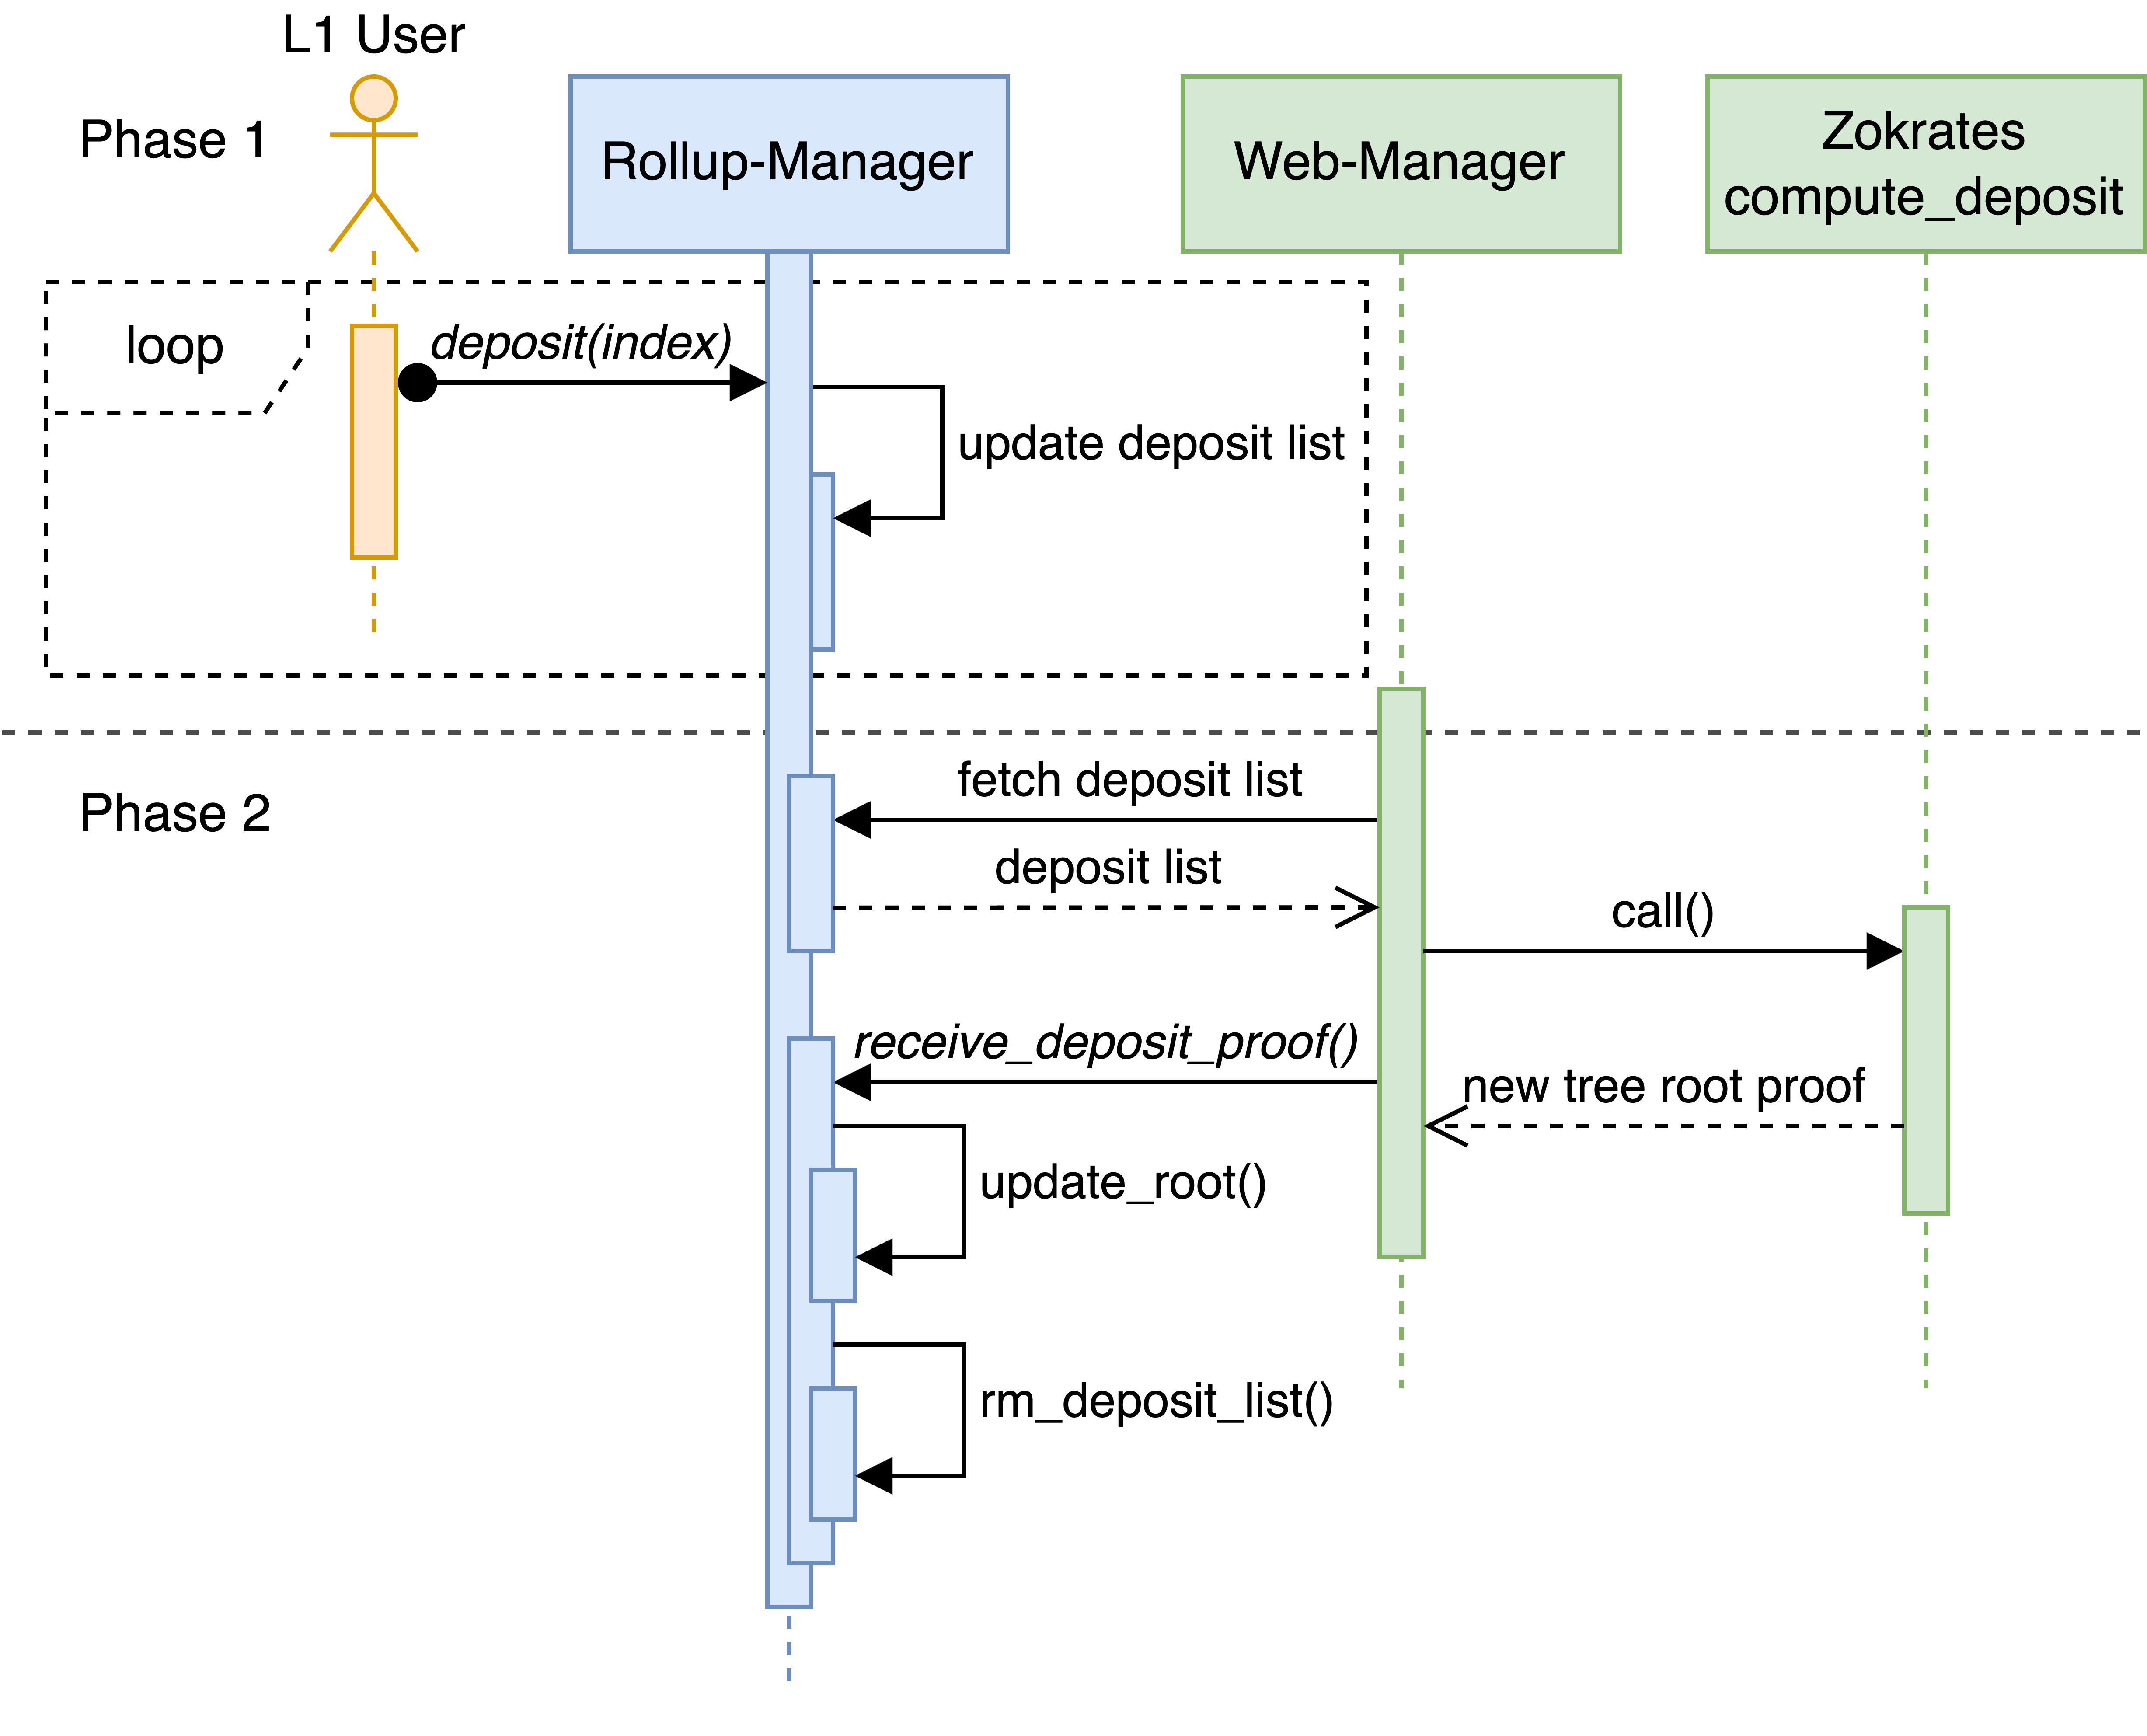
\includegraphics[width=0.7\columnwidth]{5_drawings-sequence_deposit.png}
	\caption[Sequence Deposit]{Sequence Diagram of Deposit Process}
	\label{fig:5_drawings-sequence_deposit.png}
\end{figure}

\subsection{Withdraw}
This section presents the Withdrawal process, enabling the movement of funds from the Layer 2 system to Layer 1. The withdrawal process differs from the deposit process discussed  in Section \ref{subsec:deposit}. Notably, withdrawals operate in a single phase, a strategic choice that accelerates the withdrawal procedure, enabling users to quickly retrieve their funds without the necessity of reaching a threshold of users in the withdrawal queue.

The withdrawal starts as a user sends a withdrawal request to the Web Manager. Subsequently, the Web Manager retrieves the user's balance and nonce from the manager contract and generates withdrawal inputs for the dedicated ZoKrates program. This ZoKrates program performs the computation of the new root hash for the merkle tree containing balances and nonces. This computation involves the subtraction of the user-specified amount. The computed new root hash is then sent back to the Web server. In turn, it calls the \textit{receive\_withdrawal\_proof} entrypoint within the manager smart contract providing the new root hash as parameter.

Within the manager contract, the merkle tree root hash undergoes an update, alongside adjustments to the user's balance and nonce. Subsequently, the requested sum is transferred to the user's account, finalizing the withdrawal process.

\section{Non Fungible Tokens Support}

Tezos suggests the use of the standard TZIP-12 \footnote{\url{https://tzip.tezosagora.org/proposal/tzip-12/}} for creating multi-purpose contracts able to mint tokens, including NFTs. The tokens hold some metadata, that is a map between a string and some bytes, representing strings in UTF-8. The metadata is used, for instance, to set the \textit{artifactUri}, in order to link the NFT token to the IPFS system where the artifact is stored. This simplicity allows an easy integration with the previously described Rollup System.

\subsection{Changes in Storage}

The storage of the Rollup Manager Smart Contract must be adjusted to allow storing NFT tokens. Given that NFTs can have varying quantities, it's crucial to keep track of which and how many NFTs are owned by each user. To uniquely identify a NFT a natural number is sufficient: during minting, a single number is permanently associated and represents the NFT. The primary storage change occurs in the balance field: from a natural number, it becomes a Big Map of natural numbers corresponding to the NFT ID, with their respective ownership amounts. Even with a large number of users, this change minimally affects the gas usage. As described in Section \ref{sec:5_storage} Big Maps are lazily deserialized, so only the affected tokens in a rollup are loaded in memory, saving up in gas usage.

\subsection{ZoKrates Programs}

ZoKrates Programs must also be modified to allow NFT swaps instead of regular tokens. This is possible by fetching the storage and converting the Big Map representing the state in the following way:
\begin{itemize}
	\item The nonce list remains unchanged;
	\item The inner Big Map is converted to a list of pairs, where the first element is the NFT ID and the second is the amount of NFTs owned by the user;
	\item The public key list remains unchanged.
\end{itemize}

Applying this conversion allows the ZoKrates program to have a full state of the NFTs owned by each user, and to perform swaps between users. The conversion takes place in the Web Manager, prior to sending inputs to the ZoKrates server. The number of outputs, and hence the size of the verification key, remains constant. This is made possible by the conversion and reduction mechanism described in Section \ref{sec:5_redandcompr}, which is applicable due to the free space in the field entry, previously reserved as padding. They are in fact needed 32 bit taken from the padding to represent the token type object of the transfer.

\subsection{Rollup Manager Contract}

\todo[inline]{ write about the contract changes}
